
The testing of the micromegas trigger processor and algorithm
implementation in hardware will be performed in three ways. First, in
the absence of an eight plane configuration to test the trigger, the
detector and front-end board ART output will be emulated by the
so-called  ART Pattern Generator (APG)
in order to initially characterize the system. Additionally, the trigger
system will be tested on real detectors with cosmic rays and in a
test beam.

\subsubsection{ART Pattern Generator}

In order to properly test the full trigger electronics chain without
access to a large number of chambers, it is necessary to implement a
pattern generator  to simulate the ART (address in real time) output
from  the VMM chips. This pattern generator will interface with the
ART  Data Driver Card (ADDC), which will then transmit information via
fiber optic link to the trigger processor.

The firmware for the ART Pattern Generator (APG) has been written and
is currently being tested on a Xilinx
Virtex\,7 FPGA in a VC707 development board. Each development board has
FMC output connectors. A mezzanine
card has been developed to adapt these FMC connectors to the MiniSAS
connectors expected by the ADDC card.

The signal emulation will be accomplished by reformatting simulated
muon events in the NSW in Athena and sending them via an ethernet
interface to the FPGA. On the FPGA, the hits will be sorted to the
correct ART output and clocked out according to the timing indicated
in the event. Finally, the 6 bits of the strip number are output
serially through the FMC connector according to the LVDS standard
expected by the ADDC inputs. Figure~\ref{fig:APGBlockDiag} shows the
full program flow of the APG from simulation to serialized output on
the evaluation board FPGA.

\begin{figure}[h]
 \begin{center}
 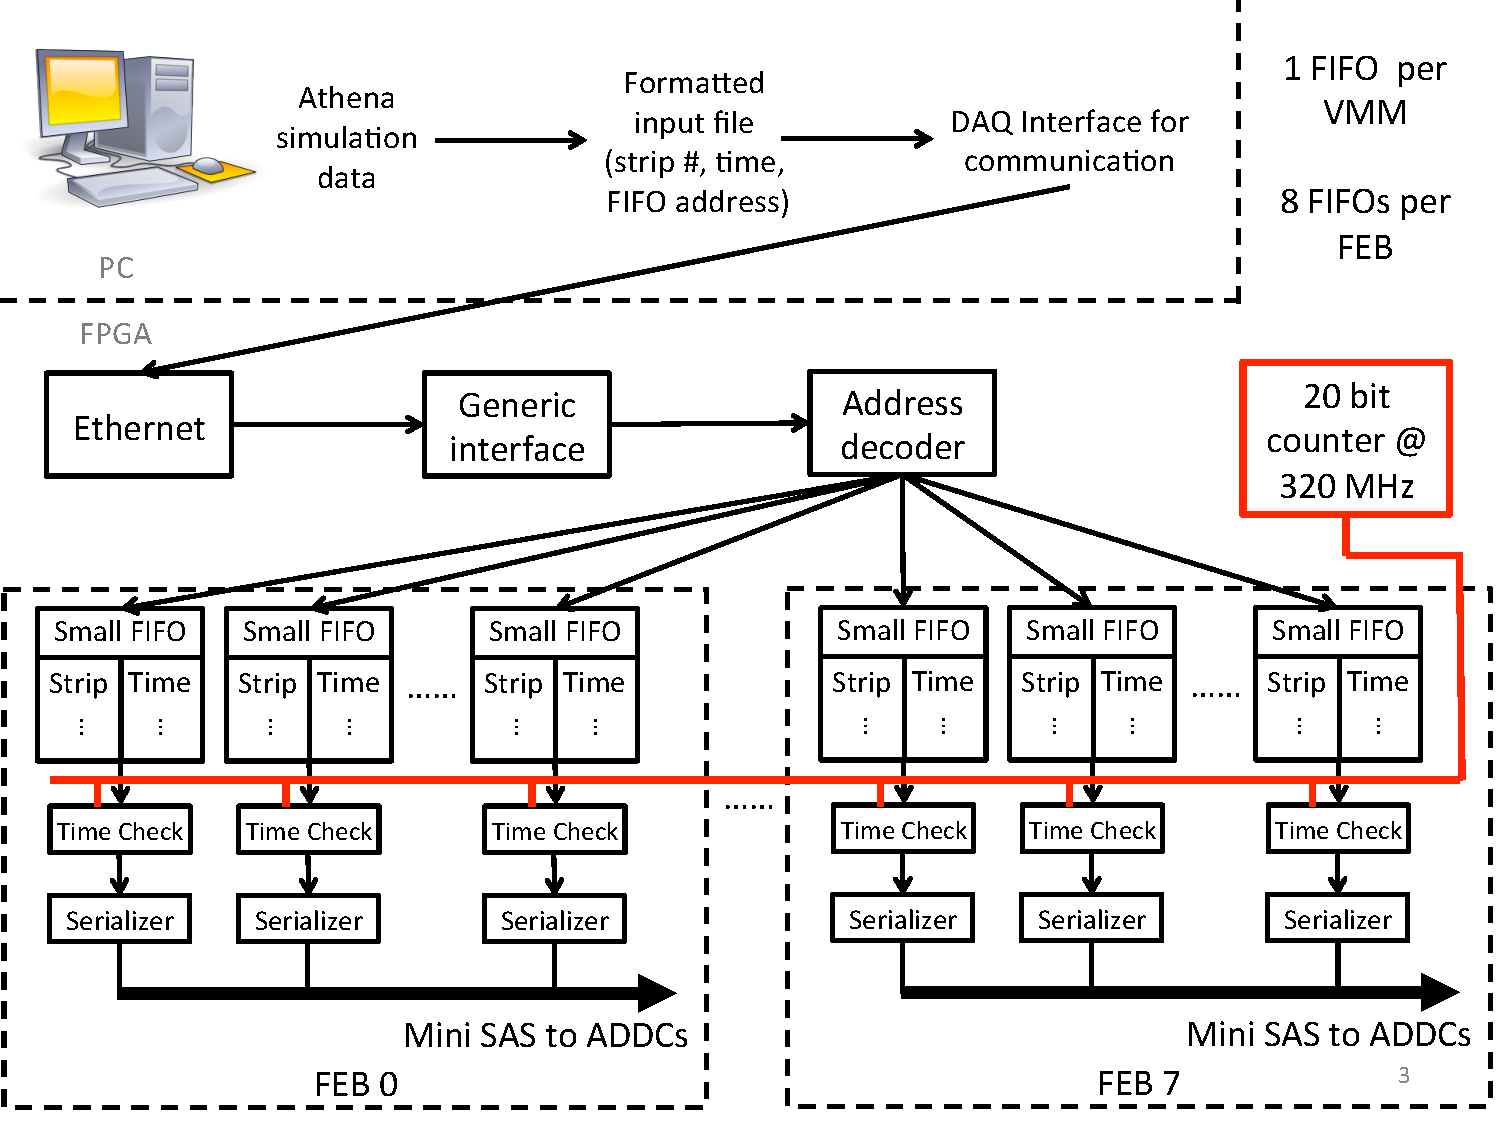
\includegraphics[width=0.8\textwidth]{figures/APGBlockDiagramFinal}
 \caption{Block diagram representing the flow of the APG}
 \label{fig:APGBlockDiag}
 \end{center}
 \end{figure}

The APG will be used in conjunction with the BNL ADDC and the trigger
processor to test the performance of the electronics and trigger
algorithm  as a function of various parameters of interest (including
track slope,  hit rates, etc.). Performance metrics for the algorithm
will include efficiency and fake rates. Performance metrics for the
electronics  will include latency measurements and stress tests with
large track and/or background rates.

\subsubsection{Testing with cosmic rays}

With real detectors available, it will be possible to do more detailed
testing of the trigger processor. Testing with cosmic rays is an
important aspect of the trigger testing plan.
A cosmic ray test stand is not subject to test beam schedules,
allowing for rapid iteration and debugging in the early stages of development.
Thus, part of the testing plan
is to assemble an eight plane micromegas configuration and place it in
a cosmic ray telescope.

It is important to ensure that
the cosmic ray muons used have sufficient momentum (O\,(1\,GeV)) so as
to avoid effects of multiple scattering. Additionally, it is useful
for the cosmic ray test setup to have a large angular acceptance, a
good angular resolution, and good timing resolution to allow precise
characterization of the trigger's behavior. One such test setup is
available at Harvard (REFERENCE?).

Once the octuplet is assembled the ultimate goal is to test the full
trigger chain with the chambers. First, the chain will be
tested with the trigger processor still in the evaluation board
platform, mainly testing the full communication pathway from chamber readout
to trigger processor. Once this is found to be working, the trigger
processor will move to its eventual home on the hardware platform in
an ATCA crate. There, more detailed tests with the cosmic rays can be
performed, including full measurements of the latency, trigger
efficiency, and hit throughput. Additionally, tests for the signal
integrity and bit errors through the whole electronics chain can be
done.

The key asset of the cosmic ray test setup is to be
able to iterate rapidly and debug issues that may arise without having
to wait for beam in a test beam setting.


\subsubsection{Test beam studies}


\subsubsection{Trigger Processor Initial Testing}

A 1/16\textsuperscript{th} slice of the complete Trigger Processor
design has been implemented and is being tested using a Xilinx VC707
Development board. This board includes a Virtex XC7VX485T-2FFG1761C
FPGA. The implementation includes 2 ADDC GBT interfaces and associated
trigger processor algorithm. 

To exercise the trigger processor design we have developed an ADDC
emulator. This design can be used to supply properly formatted ADDC
GBT packets through an optical transmitter as sent from an actual
ADDC. The same ART data used for simulations is being used for hardware
testing. We are also generating pseudo random ART data to test the
GBT communication and timing of packet decoder.

To evaluate the hardware implementation, we compare the hardware results
with results generated using a computer simulation. All of the differences
at this point are due to the number of significant bits being used
in the hardware implementation. We are currently working on optimizing
this. Figure~\ref{fig:hardwareTestingInitial} show an example of such comparisons by looking at the
differences between hardware implementation and software simulation
ROI result. in this example, the x and y axis represent the percent
error of the ROI Cartesian coordinates.

\begin{figure}[h]
 \begin{center}
 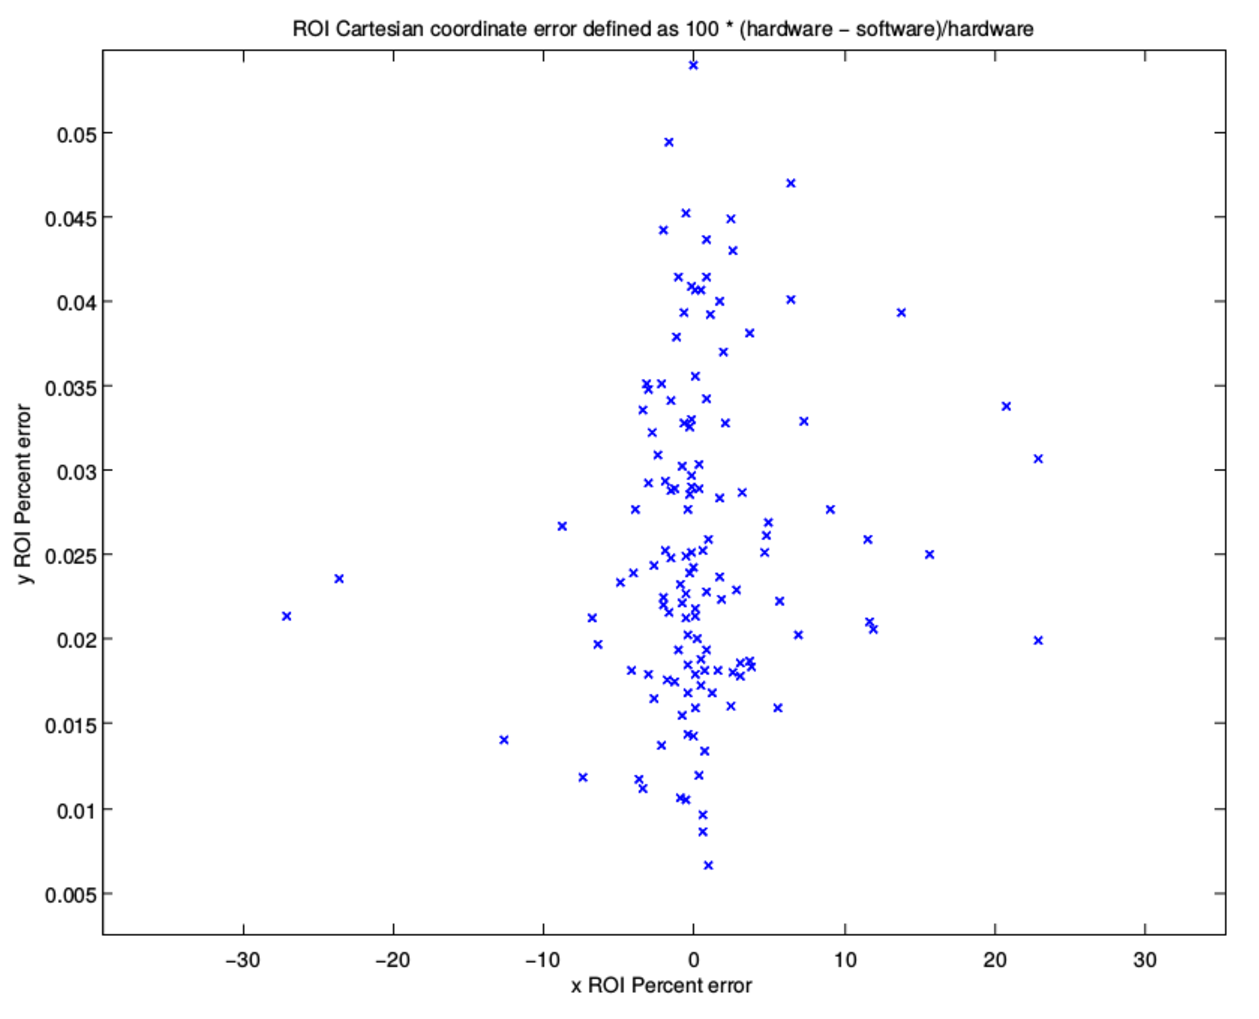
\includegraphics[width=0.8\textwidth]{figures/hardwareTestingInitial}
 \caption{Block diagram representing the flow of the APG}
 \label{fig:APGBlockDiag}
 \end{center}
 \end{figure}

We have begun integration testing with the BNL ADDC and have successfully
transmitted data to the trigger processor using the ADDC's VTRx ASIC.

